\chapter{Wave properties observed by EMFISIS and pitch angle extent of microburst}\label{appendixa}

This appendix contains Figs. \ref{B1} and \ref{B2}. Figure \ref{B1} shows evidence that supports our claim that the ``hiss-like'' chorus wave observed at 11:17:03 UT with EMFISIS WFR instrument on RBSP-A was parallel propagating. The polar angle of the wave vector and the supporting planarity of the magnetic field polarization shown in Fig. \ref{B1} was calculated using the singular value decomposition (SVD) method \citep{Santolik2003SVD}.

Figure \ref{B2} supports the claim that RBSPICE-A observed a 10-80\% increase in the count rates at the microburst times and pitch angles. Figure \ref{B2} shows the ratio of the RBSPICE-A's EBR count rates during the four microbursts to the quiet time one spin before, at the same pitch angles.

\begin{figure}
\noindent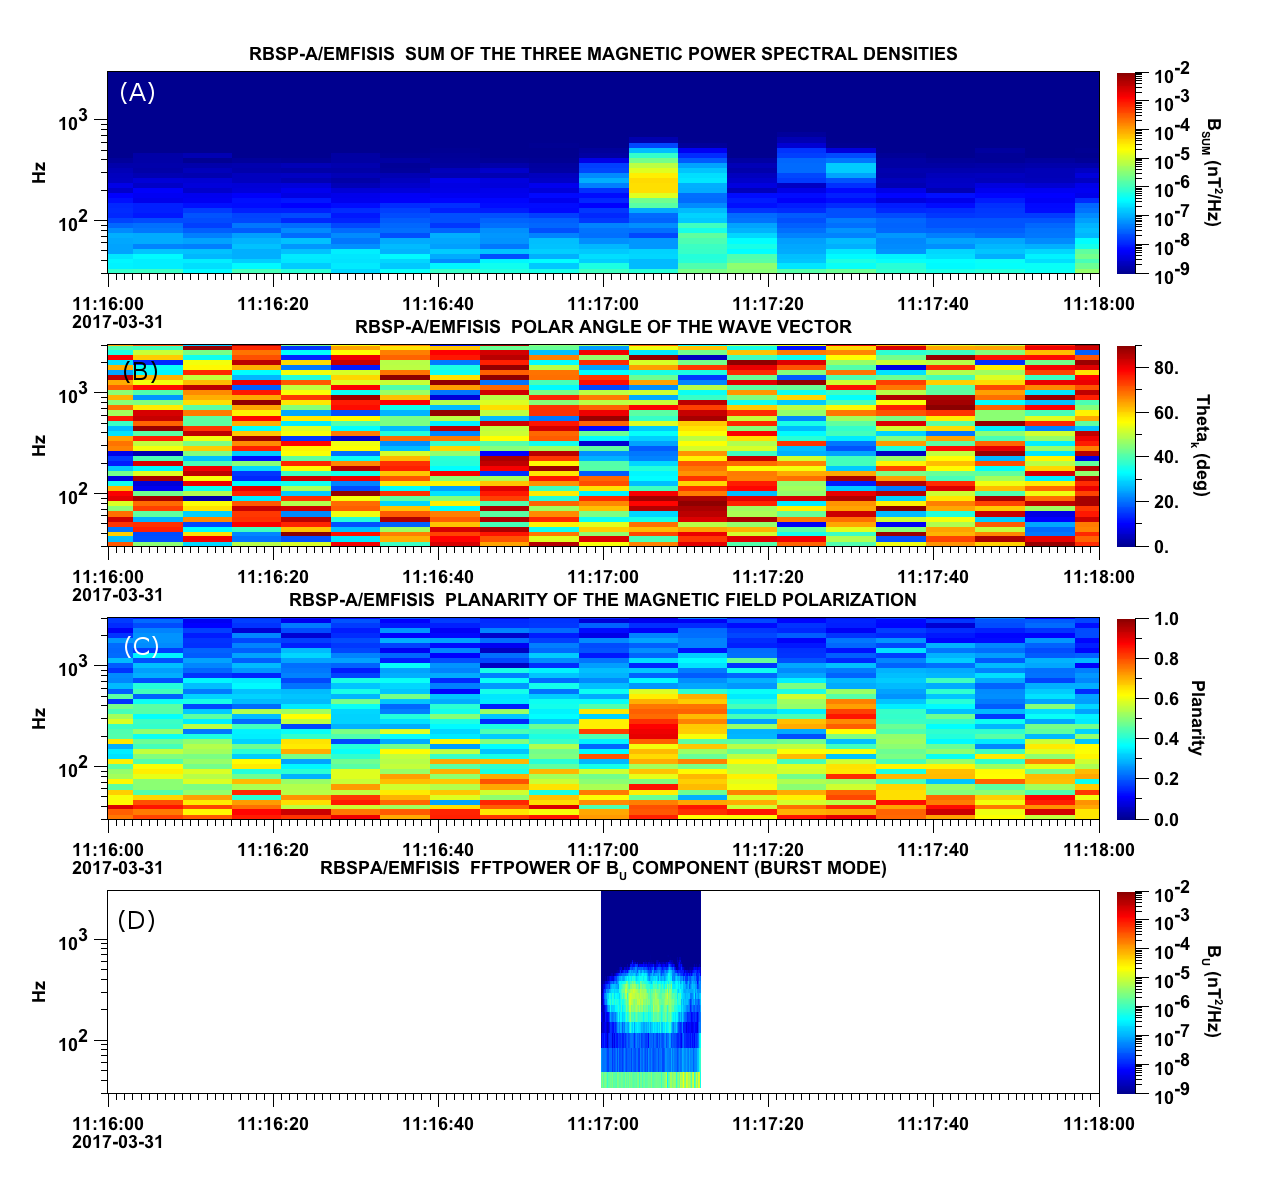
\includegraphics[width=\textwidth]{2_20170331_111600to111800_spectrogram_2.png}
\caption{Panel (A) shows the magnetic power spectral density as a function of frequency and time from the EMFISIS WFR instrument on board RBSP-A. The ``hiss-like'' wave used for the resonant diffusion analysis was observed starting at 11:17:03 UT. In the same format as panel (A), panel (B) shows the polar angle of the wave vector for this time period. The wave of interest had a normal wave vector, $\theta_k < 30^\circ$. Since the results in panel (B) are valid only for high planarity, panel (C) shows planarity in the same format as panels (A) and (B). The wave of interest was found to have a planarity of $> 0.8$. Lastly, panel (D) shows the available burst mode data.}
\label{B1}
\end{figure}

\begin{figure}
\noindent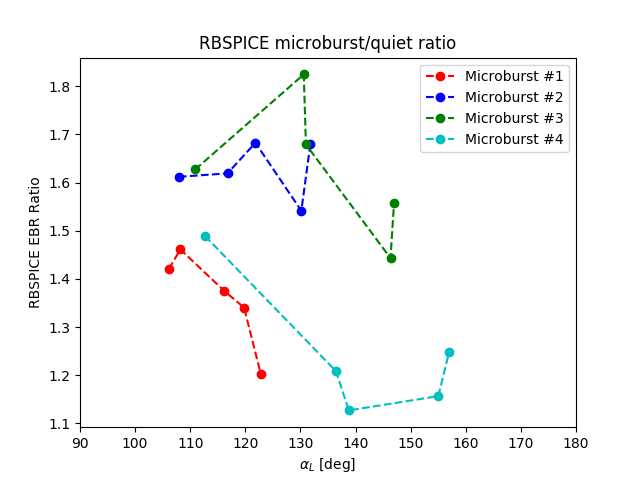
\includegraphics[width=\textwidth]{2_rbspice_pad_ratio.png}
\caption{Ratio of the RBSPICE EBR at microburst times indicated with the black vertical arrows in Fig. 2, to the EBR at the same pitch angles one spin prior (quiet time). The microburst flux was enhanced by 10-80\% across $100^\circ < \alpha_L < 160^\circ$ PA, and appear to be peaked closer to $\alpha_L = 90^\circ$.}
\label{B2}
\end{figure}